\documentclass[10pt,a4paper]{article}
\usepackage[utf8]{inputenc}
\usepackage[T1]{fontenc}
\usepackage[spanish]{babel}
\usepackage{amsmath}
\usepackage{amsfonts}
\usepackage{amssymb}
\usepackage{graphicx}
\usepackage{float}
\usepackage{subcaption}
\usepackage[colorlinks=true, citecolor=blue, final]{hyperref}
\usepackage[table]{xcolor}
\usepackage{amsmath}
\usepackage{graphicx}
\usepackage{epstopdf}

\epstopdfDeclareGraphicsRule{.gif}{png}{.png}{convert gif:#1 png:\OutputFile}
\AppendGraphicsExtensions{.gif}
\usepackage{amssymb}
\setlength{\arrayrulewidth}{1mm}
\setlength{\tabcolsep}{18pt}
\renewcommand{\arraystretch}{2.5}

\usepackage{url} % UTILIZA EL PAQUETE PARA QUE APAREZCA EL URL AUNQUE AUN NOSE SI DEBO ACTIVARLO TAMBIEN EN REFERENCIAS
\hypersetup{
    colorlinks=true,
    linkcolor=blue,
    filecolor=blue,      
    urlcolor=blue,
}
\usepackage{epsfig}
\hypersetup{colorlinks=true,
    linkcolor=blue,
    filecolor=blue,      
    urlcolor=blue,}

\usepackage{graphicx}
\usepackage[sort&compress, numbers]{natbib}
\usepackage{xcolor}
\usepackage{listings}
\usepackage{ragged2e}
\definecolor{codegreen}{rgb}{0,0.6,0}
\definecolor{codegray}{rgb}{0.5,0.5,0.5}
\definecolor{codepurple}{rgb}{0.58,1,0.82}
\definecolor{backcolour}{rgb}{1,1,0.97}
\lstdefinestyle{mystyle}{
    backgroundcolor=\color{backcolour},   
    commentstyle=\color{codegreen},
    keywordstyle=\color{magenta},
    numberstyle=\tiny\color{codegray},
    stringstyle=\color{codepurple},
    basicstyle=\ttfamily\footnotesize,
    breakatwhitespace=false,         
    breaklines=true,                 
    captionpos=b,                    
    keepspaces=true,                 
    numbers=left,                    
    numbersep=1pt,                  
    showspaces=false,                
    showstringspaces=false,
    showtabs=false,                  
    tabsize=2
}
\lstset{style=mystyle}
\usepackage{lipsum}
\usepackage{multicol}
\usepackage{xcolor}
\newcommand{\celda}[1]{
	\begin{minipage}{2cm}
		\vspace{2mm}
		#1
		\vspace{2mm}
	\end{minipage}
}
\definecolor{azul}{rgb}{0.36, 0.54, 0.66}
\usepackage[left=2.00cm, right=2.00cm, top=2.00cm, bottom=2.00cm]{geometry}
\author{Jorge Vicente Niño Mocarro}
\begin{document}
	
	\begin{figure}[H]
		\raggedright
		\includegraphics[scale=0.5]{uanl.png} \hfill \includegraphics[scale=0.275]{fime.png}
	\end{figure}

	\vspace{6mm}
	
	%ESTE CENTER ES EXCLUSIVO PARA EL TITULO DEL PAPER, AUTOR Y UNIVER.
	\begin{center}
		{\Large \textbf{Práctica 10: Algoritmo genético}}\\
		\vspace{2mm}
		\textit{ Alumno: José Adrian Garcia Fuentes}\\
		\textit{Profesor: Satu Elisa Schaeffer}\\
		\vspace{2.5mm}
		\textit{Universidad Autónoma de Nuevo León. Facultad de Ingeniería Mecánica y Eléctrica.}\\
		\vspace{1mm}
		\textit {30/abril/2021 }
		
		
	\end{center}

	\begin{center}
		\textcolor{azul}{\rule{150mm}{0.8mm}}
	\end{center}

      %ESTE ABSTRACT ES PARA EL RESUMEN PROPIAMENTE DICHO Y PARA LAS PALABRAS CLAVES (KEYWORDS) ,NOTA:el comando \par sirve para iniciar el nuevo parrafo con sangría.
	\begin{abstract}
		En esta práctica se modifica un algoritmo genético con la finalidad de resolver el problema de la mochila y se compara la mejor solución alcanzada con la solución optima obtenida con un método exacto.
		\vspace{2mm}\par
		\underline{\textbf{Palabras Claves:}} \hspace{2mm} \textit{Algoritmo, Knapsack.}
	\end{abstract}
	
	\begin{center}
		\textcolor{azul}{\rule{150mm}{0.8mm}}
	\end{center}
	
	\vspace{5mm}

	\begin{multicols}{2}
		\section{Introducción} \label{Intro}
		En la práctica 10 se utiliza el problema de la mochila este es un problema clásico de optimización particularmente de programación entera donde la tarea consiste en seleccionar un subconjunto de objetos de tal forma que no exceden la capacidad de la mochila en términos de la suma de los pesos de los objetos incluidos y que el valor total de los objetos incluidos sea lo máximo posible  \cite{p10}, mediante el problema de la mochila se implementó un algoritmo genético el cual representa posibles soluciones que satisfacen a un problema, creando valores óptimos del problema mediante una buena codificación a las diferentes variables que podrían cuantificarse para dicho método para fines de esta práctica se encontrara representado como un vector de verdadero y falso, indicando cuales objetos vamos a incluir en la mochila ($True$ o $1$ llevamos el objeto, $False$ o $0$ se descarta el objeto).

		\section{Objetivo} \label{antece}
		\begin{itemize}
		    \item Cambiar selección de mutación y de padres para reproducción a que use selección de ruleta \cite{p10}.

            \item Genere instancias con tres distintas reglas \cite{p10}.

\item Determinar para cada uno de los tres casos a partir de qué tamaño de instancia el algoritmo genético es competitivo con el algoritmo exacto  \cite{p10}.
	\end{itemize}
	\section{Metodologia}	
	La metodología empleada se realizó a través de Rstudio \cite{RStudio} llevando a cabo los pasos señalados en la \textit{Práctica 10: Algoritmo genético} \cite{p10}, a partir del código en el repositorio de Schaeffer \cite{GITSCHAEFFER}, se realizaron modificaciones. El código completo de la metodología empleada se encuentra en el repositorio de GitHub \cite{gitadrian}.
	\section{Resultados}
    Se simulo la aplicación del problema de la mochila, conocido en ingles como $Knapsack$ $problem$, donde se tienen un contenedor de capacidad $C$ limitada y se tienen $N$ elementos que se pueden meter en el contenedor , cada elemento tiene un valor de beneficio $b_i$ y un valor de capacidad $c_i$ que ocupan en el contenedor, se busca tener en el contenedor aquellos que nos maximizan el beneficio máx , donde $x_i$ es la decisión de tener o no el elemento en el contenedor sin exceder la capacidad $C$.

Se modifico la función de generador de valores tal como se muestra a continuación. 
\begin{lstlisting}
generador.valores <- function(cuantos, min, max) {
  return(sort(round(normalizar(rnorm(cuantos)) * (max - min) + min)))
}
\end{lstlisting}
Se agregaron cambios para la creación de variables.
\begin{lstlisting}
p1 <- poblacion.inicial(n, init)
p<- p1
tam <- dim(p)[1]
assert(tam == init)
pm <- sum(runif(tam) < 0.05)
rep <- 50
tmax <- 50
mejorescon <- double()
\end{lstlisting}
se crean los vectores de factibilidad y objetivos.
\begin{lstlisting}
tam <- dim(p)[1]
  obj <- double()
  fact <- integer()
  for (i in 1:tam) {
    obj <- c(obj, objetivo(p[i,], valores))
    fact <- c(fact, factible(p[i,], pesos, capacidad))
  }
\end{lstlisting}
se generan las mutaciones.
\begin{lstlisting} 
prob.mut = NULL
  for (i in 1:tam) {
    prob.mut[i] = 1/(obj[i]*(fact[i]+1)*sum(obj*(fact+1)))
  }
  mutantes<-sample(1:tam, pm, prob = prob.mut)
  for (i in mutantes) {
    p <- rbind(p, mutacion(p[i,], n)) 
  }
\end{lstlisting}
se generaron las reproducciones.
\begin{lstlisting} 
for (i in 1:tam) {
    prob.reprod[i] = obj[i]*(fact[i]+1)/sum(obj*(fact+1))
  }
 \end{lstlisting}
creacion de variables y se fabrican las interacciones del algoritmo genetico sin ruleta, aplicando una probabilidad de mutación, se determina una cantidad fija de reproducciones
\begin{lstlisting}
mejorescon <- c(mejorescon, mejor)
}
p<- p1
mejoressin <- double()
for (iter in 1:tmax) {
  p$obj <- NULL
  p$fact <- NULL
  for (i in 1:tam) {
    if (runif(1) < pm) {
      p <- rbind(p, mutacion(p[i,], n))
    }
  }
  for (i in 1:rep) { 
    padres <- sample(1:tam, 2, replace=FALSE)
    hijos <- reproduccion(p[padres[1],], p[padres[2],], n)
    p <- rbind(p, hijos[1:n])
    p <- rbind(p, hijos[(n+1):(2*n)]) 
  }
  tam <- dim(p)[1]
  obj <- double()
  fact <- integer()
  for (i in 1:tam) {
    obj <- c(obj, objetivo(p[i,], valores))
    fact <- c(fact, factible(p[i,], pesos, capacidad))
  }
  p <- cbind(p, obj)
  p <- cbind(p, fact)
  mantener <- order(-p[, (n + 2)], -p[, (n + 1)])[1:init]
  p <- p[mantener,]
  tam <- dim(p)[1]
  assert(tam == init)
  factibles <- p[p$fact == TRUE,]
  mejor <- max(factibles$obj)
  mejoressin <- c(mejoressin, mejor)
}
\end{lstlisting}

print(paste(mejor, (optimo - mejor) / optimo, optimo))
[1] "6672 0.015929203539823 6780" 

	\begin{figure}[H]
				\centering
				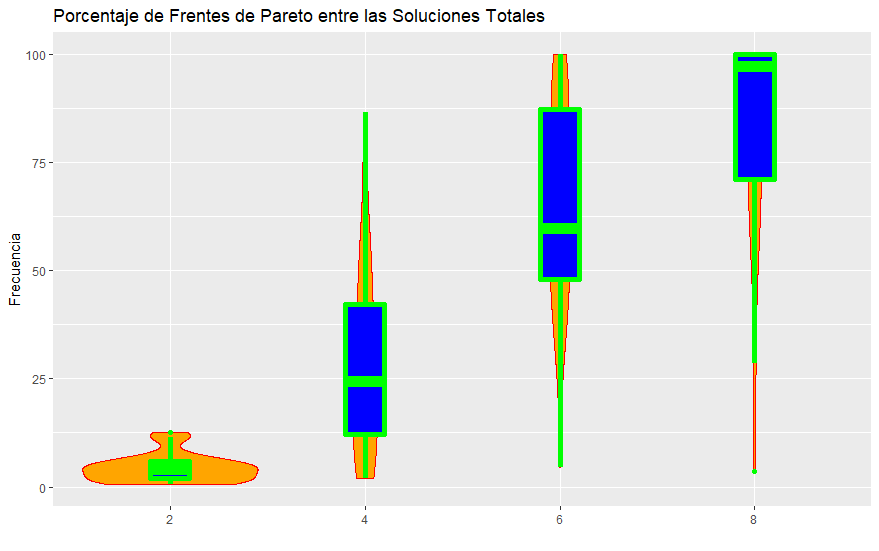
\includegraphics[scale=0.38]{Rplot.png}
				\caption{Gráfico corrplot Velocidad, Masa, Carga.}
				\label{fig: Figura1}
			\end{figure}

\begin{lstlisting}
generador.pesos <- function(valores, min, max) {
  n <- length(valores)
  pesos <- double()
  for (i in 1:n) {
    media <- valores[i]
    desv <- runif(1, max=.1)
    ruido <- rnorm(1, sd=.1)
    pesos <- c(pesos, rnorm(1, (1/media), desv) + ruido)
  }
  pesos <- normalizar(pesos) * (max - min) + min
  return(pesos)
}
\end{lstlisting}
Creacion de variables
\begin{lstlisting}
n <- 50
valores <- generador.valores(n, 10, 500)
pesos <- generador.pesos(valores, 15, 80)
\end{lstlisting}
[1] "6352 0.00235589759698445 6367"
\begin{figure}[H]
				\centering
				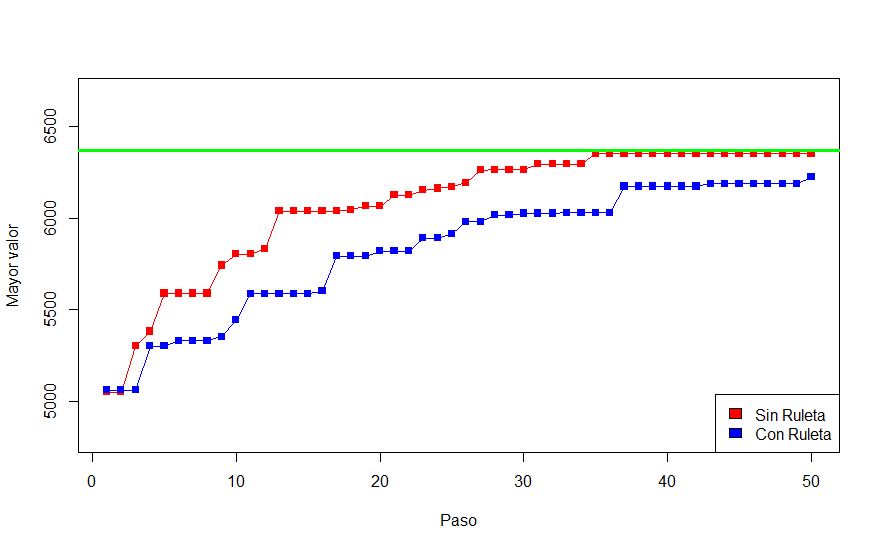
\includegraphics[scale=0.38]{Rplot012.png}
				\caption{Gráfico corrplot Velocidad, Masa, Carga.}
				\label{fig: Figura1}
\end{figure}
ultima corrida
\begin{lstlisting}
generador.valores <- function(pesos, min, max) {
  n <- length(pesos)
  valores <- double()
  for (i in 1:n) {
    media <- pesos[i]
    desv <- runif(1)
    ruido <- rnorm(1, sd=.1)
    valores <- c(valores, rnorm(1, media^2, desv) + ruido)
  }
  valores <- normalizar(valores) * (max - min) + min
  return(valores)
}
\end{lstlisting}
\begin{figure}[H]
				\centering
				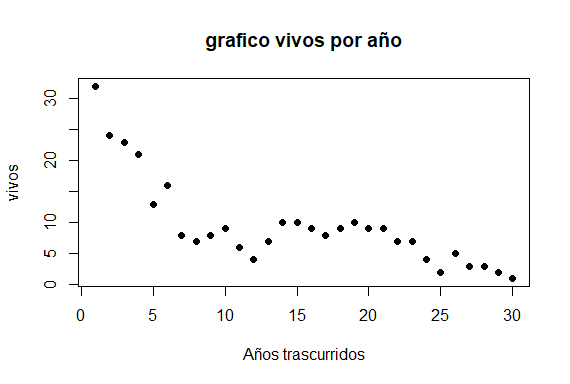
\includegraphics[scale=0.38]{Rplot01.png}
				\caption{Gráfico corrplot Velocidad, Masa, Carga.}
				\label{fig: Figura1}
\end{figure}
7417.10619389775 0.026663219978062 7620.28759843081
\section{Reto 1}
	Extender la selección de ruleta a la fase de supervivencia: en vez de quedarnos con las mejores soluciones, cada solución tiene una probabilidad de entrar a la siguiente generación que es proporcional a su valor de la función objetivo, incorporando el sí o no es factible la solución en cuestión, permitiendo que los $k$ mejores entre las factibles entren siempre (donde $k$ es un parámetro). Estudia nuevamente el efecto de este cambio en la calidad de la solución en los tres casos.
	
\begin{lstlisting}
prob.supervivencia <- NULL
\end{lstlisting}
\begin{lstlisting}
for (i in 1:tam) {
    prob.supervivencia[i] = obj[i]*(fact[i]+1)/sum(obj*(fact+1))
  }
  supervivientes<-sample(1:tam,init,prob = prob.supervivencia)
  p <- p[supervivientes,]
\end{lstlisting}
\begin{lstlisting}
for (i in 1:tam) {
    prob.supervivencia[i] = obj[i]*(fact[i]+1)/sum(obj*(fact+1))
  }
  supervivientes<-sample(1:tam,init,prob = prob.supervivencia)
  p <- p[supervivientes,]
\end{lstlisting}
\begin{figure}[H]
				\centering
				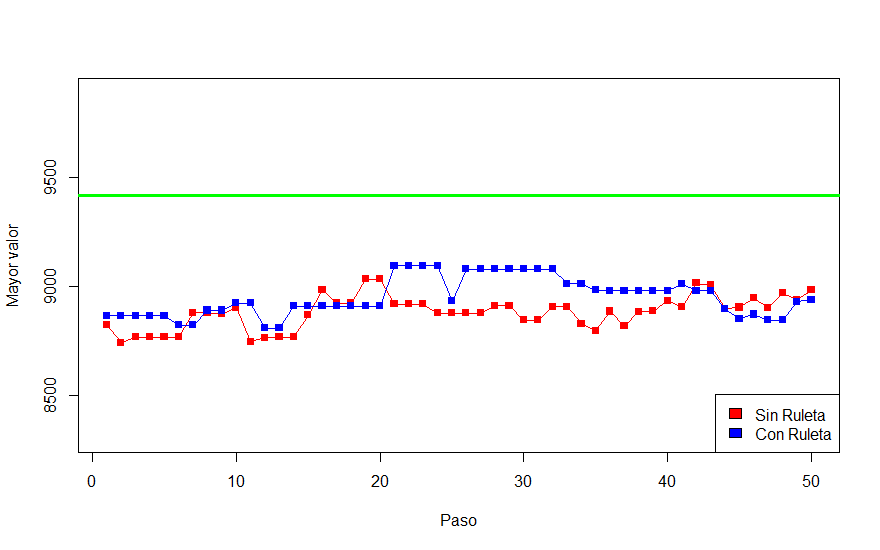
\includegraphics[scale=0.38]{reto1.1.png}
				\caption{Gráfico corrplot Velocidad, Masa, Carga.}
				\label{fig: Figura1}
\end{figure}
\begin{figure}[H]
				\centering
				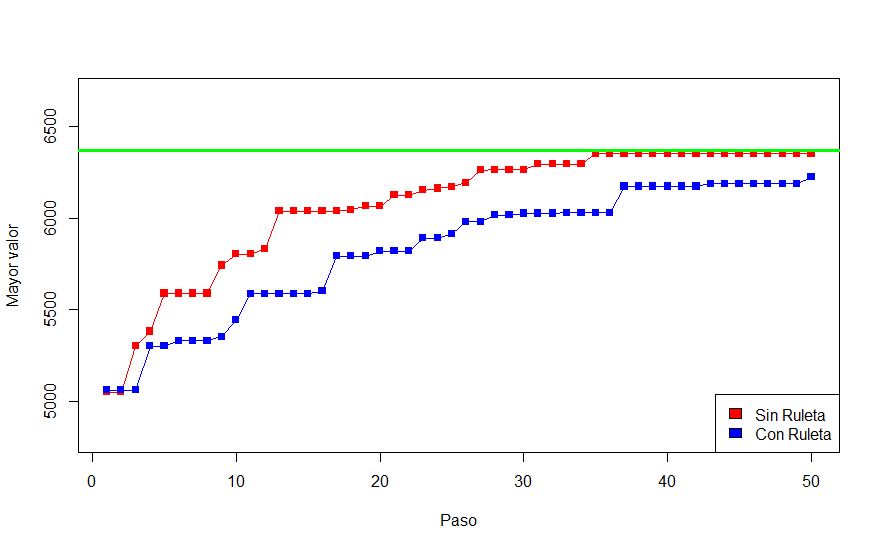
\includegraphics[scale=0.38]{Rplot012.png}
				\caption{Gráfico corrplot Velocidad, Masa, Carga.}
				\label{fig: Figura1}
\end{figure}
\begin{figure}[H]
				\centering
				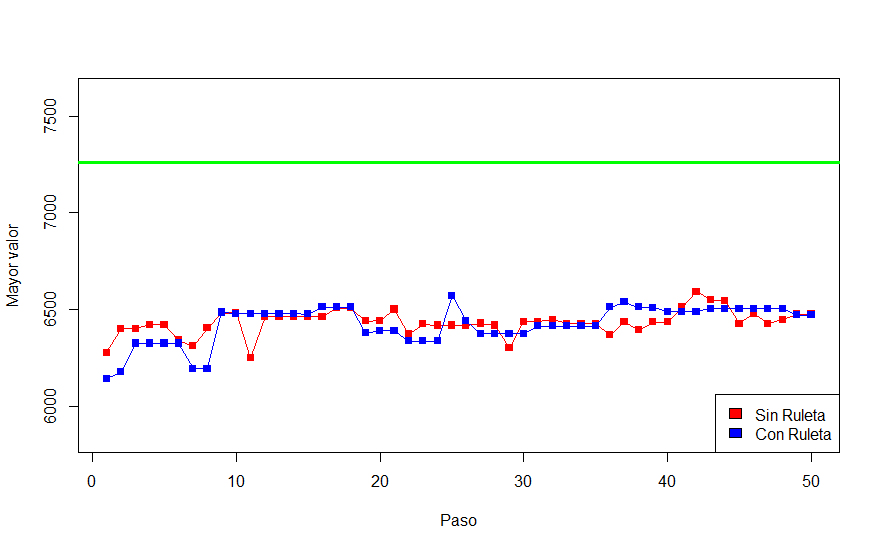
\includegraphics[scale=0.38]{Rplot13.png}
				\caption{Gráfico corrplot Velocidad, Masa, Carga.}
				\label{fig: Figura1}
\end{figure}
8982 0.0461930551130933 9417
..
4318 0.125733954241749 4939
..
6476.61404434064 0.107736061170856 7258.6302802279
	\section{Reto 2}
	Paraleliza el algoritmo genético y estudia los efectos en su tiempo de ejecución con pruebas estadísticas y visualizaciones, variando el número de objetos en la instancia.
		\section{Conclusión}
el algoritmo genético se puede mejorar al paralelizarlo, esto se nota en los tiempos de ejecución donde el tiempo de ejecución del codigo paralelizado será menor que el codigo secuencial.

\bibliography{T10}
	\end{multicols}
\bibliographystyle{ieeetr}
	
\end{document}
